\chapter{Modelo Acoplado} \label{chap:acoplado}
% CAP 6 Todo acoplado. Resultados. poner snapshots de valores 1-9

En este capítulo se realizan simulaciones de todos los fenómenos físicos simulados en los capítulos anteriores juntos, es decir el potencial eléctrico, la creación de poros en la membrana y la posterior variación en el radio de los mismos, las variaciones en la conductividad y difusión de la membrana producto de la aparición de poros y el transporte de especies iónicas en el dominio. Además se estudió el efecto de aplicar varios pulsos consecutivos a través de los electrodos, en lugar de un único pulso.

\section{Implementación}
Para realizar la simulación completa se creó un ciclo principal que realiza llamados a las diferentes rutinas implementadas en los capítulos anteriores.

Para acelerar los tiempos de ejecución se usaron intervalos temporales diferentes para los distintos fenómenos físicos simulados. Para el cálculo de la densidad y radios de los poros en la membrana celular se utilizó un intervalo temporal fijo de 1 \si{\nano\second}, ya que se notó que al aumentarlo se producen errores de discretización muy grandes que derivan en la divergencia del sistema. El cálculo del potencial eléctrico fue realizado periódicamente, a diferencia del capítulo anterior, ya que la aparición de poros afecta los valores de conductividad en la membrana y por consiguiente los potenciales eléctricos en todo el dominio. El intervalo temporal para el potencial eléctrico se eligió dinámico, con valores muy chicos al comienzo del pulso, que se hacen cada ves mayores con el paso del tiempo. Esto es porque se notó que es al principio del los pulsos que se producen cambios muy bruscos en las conductividades de la membrana celular y por lo tanto cambios en el potencial eléctrico que se deben calcular con precisión, pero que luego de un tiempo se alcanzan valores de equilibrio que no requieren intervalos temporales tan pequeños. Exactamente el intervalo temporal para el potencial eléctrico se calcula como

\begin{equation}
	\Delta_t = \mathrm{m_p} \left( 1 - e^{t/k} \right)
\end{equation}

donde $\mathrm{m_p}$ es el máximo valor de intervalo temporal posible, $t$ es el tiempo desde el inicio del último pulso y $k$ es una constante con la que se controla la velocidad con la que aumenta el intervalo temporal. En particular se utilizaron los valores de $\mathrm{m_p} = 2$ \si{\micro\second} y $k = \frac{500 \si{\micro\second}}{\ln (1 - 0.9)}$ para que el intervalo temporal aumente hacia 2 \si{\micro\second} de manera asintótica y alcance el 90\% de este valor en el instante de 500 \si{\micro\second} de comenzado el pulso. En la figura \ref{fig:deltat} se muestra el intervalo temporal en el inicio del pulso. Es importante aclarar que al comenzar y terminar cada pulso se reinicia el cálculo del intervalo temporal.

Por último se utiliza para el cálculo del transporte de especies un intervalo temporal fijo de 200 \si{\nano\second}.\\

\clearpage

\begin{figure}
	\centering
	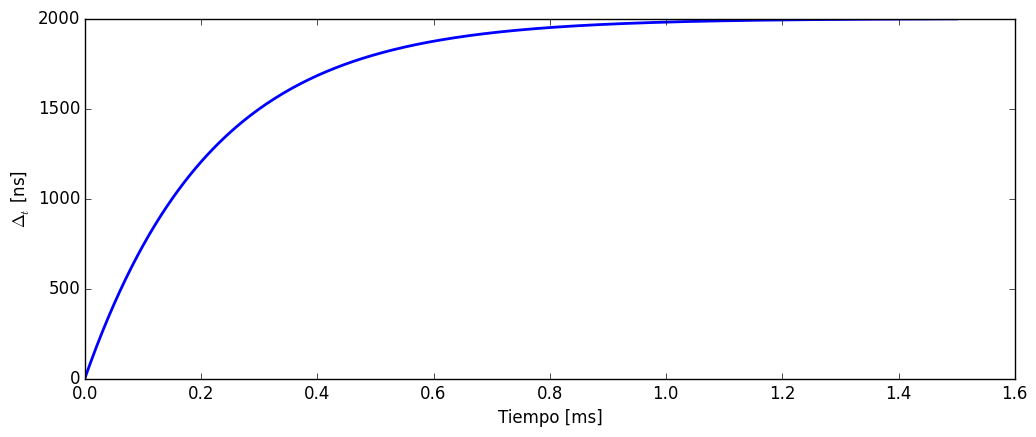
\includegraphics[width=0.8\textwidth]{acoplado/deltat}
	\caption{Intervalo temporal para cálculo del potencial eléctrico en función del tiempo desde el inicio del último pulso}
	\label{fig:deltat}
\end{figure}



% está en este capítulo aunque debería ir en poros!

%Para acelerar los tiempos de ejecución se usaron intervalos temporales diferentes para los distintos fenómenos físicos simulados. Para el cálculo de la densidad de poros en la membrana celular y sus radios se utilizó un intervalo temporal muy pequeño, ya que se notó que al aumentarlo se producen errores de discretización muy grandes que producen la divergencia del sistema. Para el cálculo de los potenciales eléctricos en el dominio, en cambio, alcanzó un intervalo temporal mucho mayor, y se notó que reducirlo no impacta en los resultados. Por último para el cálculo de las concentraciones de las especies iónicas se necesitaron intervalos temporales aún mayores. Concretamente se usaron intervalos de 1 \si{\nano\second} para las ecuaciones de poros, 20 \si{\nano\second} para el transporte de especies y un intervalo variable de entre 1 \si{\nano\second} y 2 \si{\micro\second} para el cálculo del potencial eléctrico. Este último intervalo es variable dado que los primeros instantes de cada pulso eléctrico es el que tiene mayores variaciones en los potenciales producto de la repentina permeabilización de la membrana, como puede verse en el capítulo 4. Esto hace que se necesite una actualización constante de los valores de potencial en los nodos, sobre todos los cercanos a la membrana celular. Sin embargo pasados los primeros microsegundos del pulso el sistema se estabiliza y la permeabilización y valores de PTM se mantienen con pocos cambios lo que hace innecesario un cálculo constante de los potenciales. Por esta razón se optó por un intervalo muy pequeño al comenzar un pulso y se incrementa de manera exponencial.\\

A continuación se presenta el pseudo-código del loop principal del programa. \texttt{nPulsos} es la cantidad de pulsos a simular y $\mathrm{m_p}$, $\mathrm{m_t}$ y $\mathrm{m_d}$ son constantes usadas para determinar los intervalos temporales para el cálculo de potencial eléctrico, el transporte de especies y para grabar los resultados a disco respectivamente.\\


\newcommand{\nextpoiss}{\mathtt{next}_{\mathtt{p}}}
\newcommand{\nextt}{\mathtt{next}_{\mathtt{t}}}
\newcommand{\nextd}{\mathtt{next}_{\mathtt{d}}}

\begin{algorithmic}
	\FORALL{\texttt{pulso} $\in \{1,\ldots, \mathtt{nPulsos}\}$} 
		\FORALL{\texttt{estado} $\in \{\mathtt{ON},\mathtt{OFF}\}$} 
			\STATE $t = 0$
			\STATE $\nextpoiss = \nextt = \nextd = 0$
			\WHILE{$t < \mathtt{duracion[estado]}$} 
				
				\IF{$t \geq \nextpoiss$}
					\STATE calcular potencial eléctrico con \texttt{estado}
					\STATE $\nextpoiss = t + \Delta_t \, \mathrm{m_p} \left(1 - e^{t/k}\right)$
				\ENDIF
				
				\STATE calcular densidad de poros
				\STATE calcular radios de poros
				\STATE actualizar valores de conductividad y difusión
			
				\IF{$t \geq \nextt$}
					\FORALL{$e \in \{$\h, \oh, \na, \cl$\}$} 
						\STATE calcular concentraciones de especie $e$
					\ENDFOR
					
					\STATE $\nextt = t + \Delta_t \, \mathrm{m_t}$
				\ENDIF
				
				\IF{$t \geq \nextd$}
					\STATE grabar estado en disco
					\STATE $\nextd = t + \Delta_t \, \mathrm{m_d}$
				\ENDIF								
				
				\STATE{$t = t + \Delta_t$}
			\ENDWHILE
		\ENDFOR
	\ENDFOR
\end{algorithmic}














%TODO revisar los valores de los intervalos!! revisar si transporte efectivamente mayor que poisson
%TODO mencionar truco numérico temperatura

\section{Resultados}

\subsection*{Un pulso}

\newcommand{\lineasnap}[7]{
	#2 &
	\includegraphics[width=0.19\textwidth]{#1#3.png} & 
	\includegraphics[width=0.19\textwidth]{#1#4.png} & 
	\includegraphics[width=0.19\textwidth]{#1#5.png} & 
	\includegraphics[width=0.19\textwidth]{#1#6.png} & 
	\includegraphics[width=0.19\textwidth]{#1#7.png} \\
}

Se presentan en la tabla \ref{tbl:snap1} las concentraciones en el dominio de las diferentes especies iónicas estudiadas para diferentes instantes de tiempo. Los resultados corresponden a simulaciones de una célula de 25\usec de radio bajo un pulsos eléctrico que genera un campo de 1600\vcm y una duración de 5\ms. Las imágenes de la tabla \ref{tbl:snap1} corresponden a las concentraciones molares de las cuatro especies en diferentes instantes del pulso. Los colores azules corresponden a los extremos bajos de concentración y los rojos a los extremos altos.

Se observan en todos los casos cambios en el interior de la célula mucho mayores a los obtenidos en las simulaciones del capítulo \ref{chap:trans}. Esto se debe a que la simulación de la generación de poros posibilitó la permeabilización de la membrana y el ingreso o egreso con mayor facilidad de las especies iónicas. 

En el caso del \h se observa un gran movimiento en las concentraciones, obteniéndose valores muy altos de concentración en la región hiperpolarizada del interior de la célula, que se observan con una franja roja cercana a la membrana. En cuanto a la región depolarizada del interior, la concentración de \h disminuyó notablemente, lo que se observa con una mancha de color verde que avanza hacia el ecuador de la célula con el paso del tiempo. El líquido extracelular también tuvo grandes cambios, con concentraciones altas en la región depolarizada y bajas en la región hiperpolarizada (al contrario del interior).

Las concentraciones de \oh presentan un comportamiento opuesto al observado en el \h, es decir en el interior de la célula se producen extremos altos de concentración en el polo depolarizado y una disminución de materia en el polo hiperpolarizado, mientras que en el exterior se alcanzan extremos altos cerca de la región de la membrana cercana al polo positivo y extremos bajos en el polo negativo. 

En cuanto a las concentraciones de \na y \cl, se observa mucho menos movimiento, dado que sus constantes de difusión son mucho menores que las del \h y \oh. Al igual que en los casos anteriores se tienen concentraciones extremas cerca de la membrana, con el mismo patrón de comportamiento según el signo de la especia iónica (el \na se comporta como el \h por ser de carga positiva y el \cl como el \oh por ser de carga negativa). No se observa, sin embargo, una zona de concentraciones bajas que avance hacia el centro de la célula, como en los casos anteriores, pero se alcanza a notar que las zonas con valores extremos son de mayor tamaño que las obtenidas en el capítulo \ref{chap:trans}, en el que no se tenía en cuenta la permeabilización de la membrana.

Si bien se observan cambios significativos en las concentraciones de las especies en el interior de la célula, estos cambios se dan principalmente en las regiones cercanas a la membrana. Sin embargo se observa que con el paso del tiempo las regiones con valores extremos se vuelven mayores, lo cuál indica que se podrían obtener mayores cambios en las concentraciones internas con pulsos de mayor duración o con varios pulsos. 

\begin{table}[h!] \begin{center} 
	\begin{tabular}
		{ m{0.5cm} >{\centering\arraybackslash}m{0.17\textwidth} >{\centering\arraybackslash}m{0.17\textwidth} >{\centering\arraybackslash}m{0.17\textwidth} >{\centering\arraybackslash}m{0.17\textwidth} >{\centering\arraybackslash}m{0.17\textwidth} }
		& 1\ms & 2\ms & 3\ms & 4\ms & 5\ms \\
		\lineasnap{acoplado/1p160kvm/h} {\h} {10}{20}{30}{40}{50}
		\lineasnap{acoplado/1p160kvm/oh}{\oh}{10}{20}{30}{40}{50}
		\lineasnap{acoplado/1p160kvm/na}{\na}{10}{20}{30}{40}{50}
		\lineasnap{acoplado/1p160kvm/cl}{\cl}{10}{20}{30}{40}{50}
	\end{tabular}
	\caption{Concentraciones en diferentes instantes de tiempo}
	\label{tbl:snap1}
\end{center} \end{table}

\clearpage

\subsection*{Varios pulsos}

En la tabla \ref{tbl:snap2} se presentan resultados de una simulación similar a la anterior pero con 4 pulsos de 5\ms cada uno, con un tiempo de apagado de 5\ms luego de cada pulso, en lugar de uno solo. Se utilizó la misma célula (de 25\um de radio) y el mismo potencial (1600\vcm). En todos los casos se lograron movimientos de las especies mucho mayores a los obtenidos con un solo pulso. \\

\begin{table} \begin{center} 
	\begin{tabular}
		{ m{0.5cm} >{\centering\arraybackslash}m{0.17\textwidth} >{\centering\arraybackslash}m{0.17\textwidth} >{\centering\arraybackslash}m{0.17\textwidth} >{\centering\arraybackslash}m{0.17\textwidth} >{\centering\arraybackslash}m{0.17\textwidth} }
		& 8\ms & 16\ms & 24\ms & 32\ms & 40\ms \\
		\lineasnap{acoplado/pulsos/h000} {\h} {1}{2}{3}{4}{5}
		\lineasnap{acoplado/pulsos/oh000}{\oh}{1}{2}{3}{4}{5}
		\lineasnap{acoplado/pulsos/na000}{\na}{1}{2}{3}{4}{5}
		\lineasnap{acoplado/pulsos/cl000}{\cl}{1}{2}{3}{4}{5}
	\end{tabular}
	\caption{Concentraciones en diferentes instantes de tiempo}
	\label{tbl:snap2}
\end{center} \end{table}

En las cuatro especies estudiadas se obtuvo lo siguiente:

\begin{itemize}
	\item En el interior de la célula: en todos los casos en los momentos en los que el pulso está encendido se concentran extremos altos de densidad de las especies cerca de la membrana en el hemisferio del mismo signo que la especie (es decir \h y \oh se concentran en el hemisferio hiperpolarizado y \na y \cl en el depolarizado), mientras que en el polo de signo opuesto se crea una zona con concentraciones bajas que avanzan hacia el ecuador. En cambio cuando el pulso está apagado los valores altos de concentración se dispersan desde la zona cercana a la membrana hacia el interior de la célula, aumentando así la región ocupada por concentraciones altas, mientras que la zona con concentraciones bajas deja de avanzar.

	\item En el exterior de la célula: se crea una zona de concentración alta que rodea la célula empezando en el polo de signo opuesto al signo de la especie y avanzando hacia el ecuador cuando el pulso está encendido y dispersándose y alejándose de la célula cuando el pulso está apagado. En el polo del mismo signo que la especie se observó la aparición de zonas de concentración baja que no avanzan hacia el ecuador, sino que se alejan de la célula cuando el pulso está encendido.
\end{itemize}

En el caso del \h y el \oh también se notó la aparición de zonas con concentraciones altas en el polo del mismo signo que la especie a partir del segundo pulso, provenientes del interior de la célula, mezclándose con las zonas de concentración baja, y con dirección hacia el electrodo del signo de la especie cuando el pulso está encendido. Los movimientos del \na y el \cl fueron menores que los del \h y el \oh, dada su menores constantes de difusión.\\

En la tabla \ref{tbl:chinos} se comparan valores experimentales de pH en diferentes instantes con fotografías de valores experimentales de \cite{gt99}. Los instantes de tiempo de las imágenes simuladas se eligieron para coincidir con los experimentales. En las imágenes de los experimentos se fotografiaron concentraciones de especies iónicas diferentes a las estudiadas en este trabajo. Sin embargo alcanza para observar que el proceso de ingreso de especies a la célula es similar al obtenido en las simulaciones. 

Por último se puede ver en la imagen \ref{fig:curva} que los valores de concentración se encuentran más dispersos sobre el dominio, a diferencia de los resultados obtenidos en el capítulo \ref{chap:trans}, en el que las especies se concentraban únicamente en los valores muy cercanos a la membrana y permanecían casi sin cambios en cualquier otra zona.

\begin{table} \begin{center} 
	\begin{tabular}
		{ m{0.1mm} >{\centering\arraybackslash}m{0.17\textwidth} >{\centering\arraybackslash}m{0.17\textwidth} >{\centering\arraybackslash}m{0.17\textwidth} >{\centering\arraybackslash}m{0.17\textwidth} >{\centering\arraybackslash}m{0.17\textwidth} }
		& 3.3\ms & 6.7\ms & 10\ms & 13.3\ms & 16.7\ms \\
		\lineasnap{acoplado/chinos/h} { }{1}{2}{3}{4}{5}
		\lineasnap{acoplado/chinos/gt}{ }{1}{2}{3}{4}{5}
	\end{tabular}
	\caption{Concentraciones de pH en la simulaci\'{o}n (arriba) y valores experimentales de \cite{gt99} (abajo).}
	\label{tbl:chinos}
\end{center} \end{table}

\begin{figure}
    \centering
    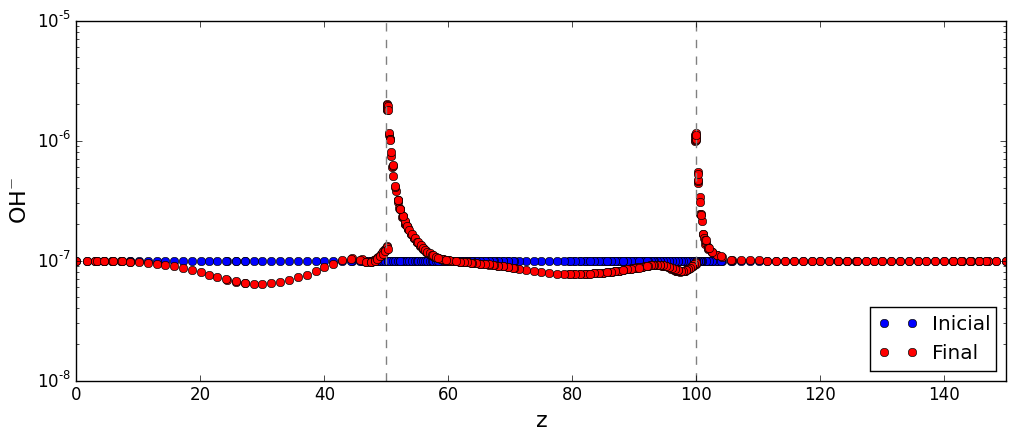
\includegraphics[width=\textwidth]{acoplado/1p160kvm/OH-321}
    \caption{Ejemplo de concentración molar de \oh en la curva de nivel $r = 2.5$ \si{\micro\metre}}
    \label{fig:curva}
\end{figure}

\clearpage
